\section{Lattice: lattice definition, base of a lattice, CVP problem, SVP problem, Hadamard ratio, Babai algorithm, GGH public key cryptosystem.}

\newcommand{\lat}{\ensuremath{\mathcal{L}}}
\newcommand{\base}{\ensuremath{\text{\textbf{B}}}}

Mřížka je sada bodů v~n-dimenzionálním prostoru s~periodickou strukturou.
V~rovině ji lze popsat kartézskými souřadnicemi $(x, y)$.
Mřížky se definují jejich bázovými vektory:
$$\lat = \lat(b_1, b_2) = \{x_1b_1 + x_2b_2 : x_i \in \mathbb{Z}\}$$

N-dimenzionální mřížka $\lat$ je množina všech celočíselných kombinaí n-lineárně nezávislých vektorů (generátorů)
$$b_1, \dots, b_n \in \mathbb{R}^n : \lat = \left\{\sum_{i=1}^n x_ib_i : x_i \in \mathbb{Z}\right\}$$

$\mathcal{B} = \{b_1, \dots, b_n\}$ se nazývá bází mřížky.
Platí že každý vektor $v \in \lat$ může být unikátně vyjářden jako lineární kombinace bázových vektorů: $v = a_1b_1 + \cdots + a_nb_n$.

V~kryptografii se využívají mřížky splňující podmínku $q \mathbb{Z}^n \subset \lat \subset \mathbb{Z}^n$ pro~některé (prvočíselné)~$q$.
Jako matice se využívá
$\base = \left( \begin{matrix}
| & | & {} & | \\
b_1 & b_2 & \cdots & b_n \\
| & | & {} & |
\end{matrix} \right);\ \lat(\base) = \{\base x : x \in \mathbb{Z}^n\}$:
například mřížka s~bázovými vektory
$b_1 = (3, 2)$, $b_2 = (1, 3)$
je zapsána jako
$\lat(\base) = \left\{\left(\begin{matrix}3&1\\2&3\end{matrix}\right)\left(\begin{matrix}x_1\\x_2\end{matrix}\right): x_1, x_2 \in \mathbb{Z}\right\}$.


\subsection{Báze mřížky}

Báze není unikátní; jedna mřížka má nekonečně mnoho kombinací bázových vektorů.

\underline{Dobrá báze} je jednoduchá na výpočty, naopak se \underline{špatnou bází} jsou výpočty komplikované a některé~problémy jsou v~nich neřešitelné; proto se dobrá báze používá jako privátní číslo a špatná báze jako veřejné číslo.
Dobré báze je blízká bázi ortogonální.

% TODO Používá se 'unimodulární' i v češtině?
Mezi bázemi je možné (jednosměrně) převádět násobením unimodulární\footnotemark{} maticí $U$.
\footnotetext{Matice je unimodulární tehdy pokud je její determinant $\pm 1$.}

\subsection{Hadamardův poměr}

Platí
$
\mathcal{H} =
\left( \frac{
| \text{det} \, \lat(v_1, \dots, v_n) | }{
|| v_1 ||_2 \cdot || v_2 ||_2 \cdot \dots \cdot ||v_n||_2
} \right)^{\frac{1}{n}}
$.
Dobrá báze má $\mathcal{H}$ blízko jedné.

% TODO Blíže vysvětlit co přesně znamená jmenovatel.
% TODO Jak vypadají špatné báze? Napsat jaké hodnoty mohou mít -- větší nebo menší?


\subsection{CVP, SVP}

\textbf{\emph{Shortest Vector Problem}}: pro~zadanou mřížku $\lat$ najděte nejkratší nenulový vektor $v$ z~$\lat$ s~minimální velikostí $||v||_2$.
V~současnosti neexistuje žádný algoritmus s~polynomiální složitostí.
Existují deterministické ($n^{O(n)}$)\footnotemark{} či randomizované ($2^{O(n)}$)\footnotemark{}; rychlejší nejsou pravděpodobné, protože jde o~NP-hard problém.
\footnotetext{Kannan, Ravi (1983): Improved Algorithms for Integer Programming and Related Lattice Problems \\ \url{https://doi.org/10.1145/800061.808749}}
\footnotetext{Ajtai, Miklós; Kumar, Ravi; Sivakumar, D. (2001): A sieve algorithm for the shortest lattice vector problem \\ \url{https://doi.org/10.1145/380752.380857}}

\emph{Worst-case} SVP je možné redukovat na~\emph{average-case}\footnotemark{}.
\footnotetext{Ajtai, Miklós (1998): The shortest vector problem in L2 is NP-hard for randomized reductions. \\ \url{https://doi.org/10.1145/276698.276705}}
Nejde o~problém dostatečně složitý pro~praktickou kryptografii.

\textbf{\emph{Closest Vector Problem}}: pro~zadanou mřížku $\lat$ a vektor $t \in \mathbb{R}^n$ najděte nenulový vektor $v \in \lat$ takový abyste minimalizovali $||t - v||_2$.
Existuje deterministický algoritmus ($n^{O(n)}$)\footnotemark{}.
\footnotetext{Micciancio, Daniele; Voulgaris, Panagiotis (2010): Faster Exponential Time Algorithms for the Shortest Vector Problem \\ \url{https://doi.org/10.1137/1.9781611973075.119}}

Jinými slovy jde o~prohledávání okolí vektoru a~nalezení bázového vektoru který je k~hledanému nejbližší.
Jde o~generalizaci SVP.
CVP$_\gamma$: vzdálenost může být nejvýše $\gamma$ (tzv. aproximační faktor).
Platí že $\gamma$-GapCVP' je NP-hard pro~$\gamma \ge 1$\footnotemark{}.
\footnotetext{Arora, S., L. Babai, J. Stern, and E.Z. Sweedyk (1997). The hardness of approximate optima in lattices, codes, and systems of linear equations}


\subsection{Babaiův algoritmus}

Pokud je $\base$ ortogonální báze v~$\lat$, approx-CVP může být vyřešen v~polynomiálním čase.
Algoritmus funguje i při~dostatečně ortogonálních bázích.

\begin{enumerate}
\item $t = t_1 b_1 + t_2 b_2 + \cdots + t_n b_n$ kde $t_1, t_2, \dots, t_n \in \mathbb{R}$.
\item $v = a_1 b_1 + a_2 b_2 + \cdots + a_n b_n$ kde $a_i = \lceil t_i \rfloor$ pro $i = 1, 2, \dots, n$.
\end{enumerate}

% FIXME Vysvětlení?

\begin{figure}[ht]
    \emph{Příklad}: Pro $t = (-1.1, 6.2)$ získejte $v$.

    \begin{minipage}{0.5\textwidth}
        \centering
        \caption*{\emph{dobrá báze:}}

        $b_1 = (5, 0)$, $b_2 = (1, 2)$

        $t_1\left(\begin{matrix}5\\0\end{matrix}\right) + t_2 \left(\begin{matrix}1\\2\end{matrix}\right) = \left(\begin{matrix}-1.1\\6.2\end{matrix}\right)$

        $v = -b_1 + 3b_2 = (-2, 6)$
    \end{minipage}\hfill\begin{minipage}{0.5\textwidth}
        \centering
        \caption*{\emph{špatná báze:}}

        $b_1 = (9, 8)$, $b_2 = (8, 6)$

        $t_1\left(\begin{matrix}9\\8\end{matrix}\right) + t_2 \left(\begin{matrix}8\\6\end{matrix}\right) = \left(\begin{matrix}-1.1\\6.2\end{matrix}\right)$

        $v = 6b_1 - 7b_2 = (6, 12)$
    \end{minipage}
\end{figure}


\subsection{Asymetrický kryptosystém GGH}

Alice vybírá lineárně nezávislé vektory $v_1, v_2, \dots, v_n \in \mathbb{Z}^n$ které jsou k~sobě celkem kolmé (což lze zjistit Hadamardovým poměrem).
Vektory $v_i$ jsou Alicin privátní klíč (uspořádán do~řádků v~$n \times n$ matici $V$).

Alice vytvoří $n \times n$ matici $\textbf{U}$ tak aby $\text{det}(\textbf{U}) = \pm 1$.
Poté spočítá $\textbf{W} = \textbf{UV}$.
Řádky matice $\textbf{W}$ ($w_1, \dots, w_n$) je nová báze $\lat$ a Alicin veřejný klíč.

Pro~poslání zprávy vybere Bob malý vektor $m$ s~celočíselnými souřadnicemi.
Vybere také náhodný rušivý vektor $r$ (např. z~předem definovaného rozsahu $-\delta$ až $\delta$) a vypočítá
$e = m\textbf{W} + r = \sum_{i=1}^n m_i w_i + r_i$.

Alice použije Babaiův algoritmus se~svou dobrou bází $v_1, \dots, v_n$ k~nalezení vektoru v~$\lat$ blízkému $e$.
Protože používá dobrou bázi a~$r$ je malé, vypočítá $m\textbf{W}$.
Tuto hodnotu vynásobí $\textbf{W}^{-1}$ a tím získá $m$.

Jde o~schéma bezpečné, ale kvůli velikosti bezpečnostních parametrů nepraktické.
(Převzato z~\emph{An Introduction to Mathematical Cryptography}\footnotemark{}).
\footnotetext{\url{https://staff.emu.edu.tr/alexanderchefranov/Documents/CMSE491/CMSE491 Fall2020/Hoffstein2015 Introduction to Mathematical Cryptography 409-412 GGH.pdf}. \\ Plně dostupné na \url{https://doi.org/10.1007/978-1-4939-1711-2}}


\clearpage
\section{LWE and RLWE: LWE problem, RLWE problem, Regev one-bit cryptosystem.}

Všechny LWE problémy jsou do~určité míry ekvivalentní (pro~rovnou bezpečnost může být nutné upravit bezpečnostní parametry).
V~praxi proti nim neexistuje útok.

Obecně jde o~řešení problému soustavy rovnic.
Samotná matice lze řešit Gaussovskou eliminací, ale po~přidání chyby $e \in \{-1, 0, 1\}$ k~výsledkům již správný výsledek vycházet nebude.

$$
\left[
\begin{matrix}
1 & 5 & 3 & 2 \\
1 & 4 & 2 & 6 \\
2 & 1 & 3 & 1 \\
3 & 4 & 4 & 6 \\
\end{matrix}
\right] \equiv \left[
\begin{matrix}
1 \\ 2 \\ 4 \\ 0
\end{matrix}
\right] + e
\equiv \left[
\begin{matrix}
{\color{gray}1+1=}\, 2 \\
{\color{gray}2+0=}\, 2 \\
{\color{gray}4-1=}\, 3 \\
{\color{gray}0-1=}\, 6 \\
\end{matrix}
\right] \pmod 7
$$


\subsection{Learning with Errors}

LWE lze zapsat jako $\textbf{A}s + e = b$. Obsahuje $n$ polynomů (řádu $m$), tajemství $s$ a chybu $e$.

$s$ je nalezitelné linearizací pokud je $\chi$ náhodně rozložené v~$\mathbb{Z}_2$ (tj. $n=1$ a $e \in \{-1, 0, 1\}$).
Bezpečnost tedy závisí na~volbě distribuce $\chi$.

Je možné ho uplatit na~symetrické i asymetrické šifrování, výměnu klíčů, digitální podpisy, (plně) homomorfní šifrování, ZK protokoly a další.

\subsection{Ring Learninig with Errors}

LWE trpí velikostmi klíčů ($n^2$).
R-LWE redukuje matici \textbf{A} na~jediný řádek, který je pokaždé horizontálně posunutý o~jednu pozici vpravo.
Stačí tak přenášet pouze tento jeden řádek a ne~celou matici.
Vytvořená struktura je ideální mřížka, ve~které může být grupa $\mathbb{Z}_q^n$ nahrazena polynomiálním okruhem $\mathbb{Z}_q[x]/\left<x^n+1\right>$.

R-LWE lze zapsat jako $\textbf{A} + s \equiv b$. Obsahuje $n$ polynomů (řádu $m$) a tajemství $s$.

Redukce na~polynomy výrazně zmenšuje velikost přenášených klíčů $\textbf{A}, s$.

\subsection{Regev one-bit kryptosystém}

\begin{wrapfigure}{r}{16em}
    \centering
    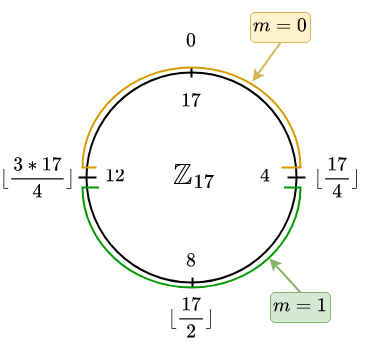
\includegraphics[width=13em]{regev}
\end{wrapfigure}

Schéma stavící na~LWE.
Privátním klíčem je $s$, $e$, veřejným $A$, $b$.

Chceme zašifrovat jednobitovou zprávu $m$.
V~určité grupě ($\mathbb{Z}_{17}$) můžeme zvolit $p$ takové aby $c = p+m$ šumem nepřerušilo zprávu.

V~našem konkrétním případě $\mathbb{Z}_{17}$ může být šum maximálně $\pm \frac{17}{4}$.
Dešifrováno bude $\begin{cases}
1: & p \in \left<5, 11\right> \\
0: & p \in \left<-4, 3\right> \\
\end{cases}$.

% NOTE Zde je možné přidat schéma/obrázek z prezentace (Post-Quantum Cycles, slide 28)


\clearpage
\section{Lattice-based protocols: Module-LWE problem, LWR problem, NTT, KYBER scheme, SABER scheme.}

\subsection{M-LWE}

Modul je generalizace tělesa, ve~kterém je těleso\footnotemark{} nahrazeno okruhem\footnotemark{}.
\footnotetext{Těleso je okruh který obsahuje inverzní prvky vzhledem k~násobení.}
\footnotetext{Okruh je uzavřený, asociativní, komutativní, distributivní, obsahuje nulový a inverzní prvky vzhledem ke~sčítání.}
M-LWE je jednodušší struktura než R-LWE a je rychlejší než LWE.

Pro~M-LWE platí, že je obtížné získat tajný vektor $s$ při~znalosti matice \textbf{A} a~vektoru $b$, kde
$$
b =
\textbf{A}s + e =
\left(\begin{matrix}
a_{11}(x) & a_{12}(x) & a_{13}(x) \\
a_{11}(x) & a_{12}(x) & a_{13}(x) \\
a_{11}(x) & a_{12}(x) & a_{13}(x) \\
\end{matrix}\right) \left(\begin{matrix}
s_{11}(x) \\ s_{21}(x) \\ s_{31}(x) \\
\end{matrix}\right) + \left(\begin{matrix}
e_{11}(x) \\ e_{21}(x) \\ e_{31}(x) \\
\end{matrix}\right)
$$

Chyba $e$ je vytvořena násobením nebo zaokrouhlováním.
% TODO Vysvětlit do větších detailů

% TODO Vysvětlit co se zde děje, je to šifrování?
% TODO V čem je důležité to že je to polynomiální modulus?
Nechť $q$ je polynomiální modulus a $p < q$.
Poté $b = \lfloor \frac{p}{q} \textbf{A}s \rfloor$.
Zaokrouhlováním dolů se chyba stává deterministická.
Pokud jsou $p$ a $q$ mocniny dvou, operace násobení a zaokrouhlování jsou velmi rychlé.

% TODO Jak dešifrovat?

\subsection{LWR}
% Learning with Rounding, Revisited. New Reduction, Properties and Applications
%  https://www.iacr.org/archive/crypto2013/80420212/80420212.pdf

\emph{Learning with Rounding} je varianta LWE, kde je náhodná chyba nahrazena deterministickým zaokrouhlováním.
Jde o~problém postavený na~Regev a je stejně těžký jako LWE.

Pro~$p < q$ rozdělíme prvky $\mathbb{Z}_q$ do~$p$ sousedících intervalů (každých velkých zhruba $q/p$), a definujeme funkci zaokrouhlení $\lfloor \cdot \rfloor_p$: $\mathbb{Z}_q \rightarrow \mathbb{Z}_p$ která mapuje $x \in \mathbb{Z}_q$ na~index intervalu do~kterého $x$ patří.

LWR tvrdí že $(\textbf{A}, \lfloor \textbf{A} \cdot s \rfloor_p)$ je výpočetně nerozlišitelné od~$(\textbf{A}, \lfloor b \rfloor_p)$, kde $b$ je veřejný vektor.

% TODO Nalinkovaný paper obsahuje spoustu informací o bezpečnosti parametrů, hodilo by se tu něco z toho mít?

\subsection{NTT}
\label{sec:ntt}

\emph{Number Theoretic Transform} je specializace diskrétní Fourierovy transformace na~okruhu.
Inverzní NTT odpovídá rekonstrukci původního polynomu při~znalosti několika jeho bodů:

$$
b(x):
\left[\begin{matrix}
3 \\ 0 \\ 0
\end{matrix}\right] = \left[\begin{matrix}
1 & 1 & 1 \\ 4 & 2 & 1 \\ 1 & 4 & 1 \\
\end{matrix}\right]
\hspace*{1em}
\mathrel{\mathop{\longrightarrow}^{\text{deg}(b)=5}_{\in \, \mathbb{Z}_5[x]}}
\hspace*{1em}
b(x) = x^2 - x + 3
$$

\subsection{Dohoda na~sdíleném klíči v~LWE schématu}

\begin{table}[ht]
    \centering
    \begin{tabular}{ccc}
    Alice & & Bob \\
    \hline
    vytvoření $s_a$, $e_a$ & & vytvoření $s_b$, $e_b$ \\
    $b_a = As_a + e_a$ & & $b_b = A^Ts_b + e_b$ \\
    & $\stackrel{b_a}{\longrightarrow} \ \ \stackrel{b_b}{\longleftarrow}$ & \\
    $v_a = s_a^T b_b$ & & $v_b = s_b^T b_a$ \\
    & $v_a \approx v_b^T$ & \\
    \end{tabular}
\end{table}
\FloatBarrier

\subsection{KYBER}

CRYSTALS-Kyber je KEM schéma založené na~mřížkách.
Je založené na M-LWE a je post-kvantově bezpečné.
Je to (jediný) výherce třetího kola soutěže PQC NIST.

Náročnost (\emph{security levels}) lze upravovat změnou velikosti \textbf{A} (počtu polynomů) a náhodného rozložení.
Pokud je chyba moc velká, dešifrování se nemusí podařit, ale pravděpodobnost takového stavu je pouze malá ($< 2^{100}$).

\subsection{SABER}

Saber je KEM schéma založené na~mřížkách.
Je založené na~M-LWE a je post-kvantově bezpečné.
Byl to kandidát třetího kola PQC NIST.

\begin{figure}[ht]
    \centering
    \begin{minipage}[t]{0.5\textwidth}
        \centering
        \caption*{KYBER}

        \begin{tabular}{lcr}
        \textbf{Vytvoření klíčů} && \\
        $s_a \leftarrow \text{random()}$ && \\
        $\textbf{A} = \text{gen}(s_a)$ && \\
        $s = \text{gen()}$ && \\
        $e = \text{gen()}$ && \\
        $b = \textbf{A}^T s + e$ && \\
        & $\stackrel{s_a, b}{\longrightarrow}$ & \\
        && \textbf{Šifrování} \\
        && $\text{zpráva}\ m$ \\
        && $\textbf{A} = \text{gen}(s_a)$ \\
        && $s' = \text{gen()}$ \\
        && $e' = \text{gen()}$ \\
        && $b' = \textbf{A}s' + e'$ \\
        && $c = b^Ts' + \frac{q}{2}m$ \\
        & $\stackrel{b', c}{\longleftarrow}$ & \\
        \textbf{Dešifrování} && \\
        $v = b'^T s$ && \\
        $m = \frac{2}{q}(c - v)$ && \\
        \end{tabular}
    \end{minipage}\hfill\begin{minipage}[t]{0.5\textwidth}
        \centering
        \caption*{SABER}

        \begin{tabular}{lcl}
        \textbf{Vytvoření klíčů} && \\
        $s_a \leftarrow \text{random()}$ && \\
        $\textbf{A} = \text{gen}(s_a)$ && \\
        $s = \text{gen()}$ && \\
        $b = \lfloor \frac{p}{q} \textbf{A}^T s \rceil$ && \\
        & $\stackrel{s_a, b}{\longrightarrow}$ & \\
        && \textbf{Šifrování} \\
        && $\text{zpráva}\ m$ \\
        && $\textbf{A} = \text{gen}(s_a)$ \\
        && $s' = \text{gen()}$ \\
        && $b' =\lfloor \frac{p}{q} \textbf{A} s' \rceil$ \\
        && $c = \lfloor \frac{T}{q} b^T s' + \frac{T}{2} m \rceil$ \\
        & $\stackrel{b', c}{\longleftarrow}$ & \\
        \textbf{Dešifrování} && \\
        $v = b'^T s$ && \\
        $m = \lfloor \frac{2}{q} (v - \frac{p}{T} c) \rceil$ && \\
        \end{tabular}
    \end{minipage}

    \vspace*{1em}
    V~ukázkách výše všechny polynomy náleží do~$\mathbb{Z}_q[x]/(x^{256}+1)$.
\end{figure}

\begin{table}[ht]
    \centering
    \begin{tabular}{|l|l|}
    \textbf{Kyber} & \textbf{Saber} \\
    \hline \hline
    prvočíselné modulo & modulo mocniny dvou \\
    je vyžadován NTT solver & flexibilní multiplikační algoritmus \\
    softwarově efektivní & hardwarově efektivní \\
    \end{tabular}
\end{table}


\clearpage
\section{Homomorphic Encryption (HE): homomorphism, HE definition, kind of HE (partially, somewhat, fully), Bootstrapping, Paillier Cryptosystem}

Homomorfismus je zobrazení z~jedné algebraické struktury do~jiné stejného typu, které zachovává důležitou strukturu.
y
Šifrovací schéma $E$ je homomorfní pokud platí $f(E(x)) = E(f(x))$:
\begin{align*}
    E_k(a) \oplus_c E_k(b) &= E_k (a \oplus_p b)
    \\
    E_k(a) \otimes_c E_k(b) &= E_k(a \otimes_p b)
\end{align*}
\noindent
kde $(P, \oplus_p, \otimes_p)$ a $(C, \oplus_c, \otimes_c)$ jsou \emph{plaintext} a \emph{ciphertext} prostory a $a, b \in P$ dvě zprávy.

Umožňuje provádět operace s~daty bez~toho aby bylo nutné je dešifrovat (tj. bez znalosti privátního klíče); dešifrováním se získá výsledek operací, který by byl získán i~kdyby operace proběhly nad~dešifrovanými daty.

\subsection{Druhy homomorfního šifrování}

% https://dspace.cvut.cz/handle/10467/101730, str 6

\textbf{Částečně homomorfní šifrování} (\emph{Partially Homomorphic Encryption}) podporuje pouze jednu z~operací (sčítání nebo násobení).
Cesarova šifra umožňuje homomorfické sčítání, RSA a ElGamal (v~surové matematické formě) umožňují homomorfické násobení.

\textbf{Celkem homomorfní šifrování} (\emph{Somewhat Homomorphic Encryption}) podporuje obě operace, ale pouze pro~omezený počet operací.

\textbf{Vyrovnané plně homomorfní šifrování} (\emph{Leveled Fully Homomorphic Encryption}) podporuje více operací do~předem daného počtu operací.

\textbf{Plně homomorfní šifrování} (\emph{Fully Homomorphic Encryption}) podporuje více operací při~libovolném počtu operací.

\subsection{Bootstraping}

Při~provádění operací roste šum. Šumem je malé číslo $r$ díky kterému není kryptosystém náchylný na~rozbití GCD (protože $c_1 = pq_1 + 2r_1 + m$ a $c_2 = pq_2 + 2r_2 + m$ sdílí $p$ jako GCD):

\begin{table}[ht]
    \centering
    \begin{tabular}{lcr}
    \textbf{Vytvoření klíčů} && \\
    $p \in_\mathbb{N} [2^{k-1}, 2^k]$ \\
    & $\stackrel{p}{\rightarrow}$ & \\
    && \textbf{Šifrování} \\
    && zpráva $m \in \{0,1\}$ \\
    && $q \in \mathbb{N}$ \\
    && $r \in_\mathbb{R} [2^{k-1}, 2k], |2r| < |\frac{p}{2}|$ \\
    && $c = pq + 2r + m$ \\
    & $\stackrel{c}{\leftarrow}$ & \\
    \textbf{Dešifrování} && \\
    $m = (c \mod p) \mod 2$ && \\
    \end{tabular}
\end{table}
\FloatBarrier

Šum je $2x$-násobný po~sčítání a $x^2$-násobný po~násobení:
\\XOR: $c_1 + c_2 = p(q_1 + q_2) + 2(r_1 + r_2) + (m_1 + m_2)$
\\AND: $c_1 c_2 = p(c_2 q_1 + c_1 q_2 - q_1 q_2) + 2(r_1 r_2 + r_1 m_2 + r_2 m_1) + m_1 m_2$


\emph{Bootstrapping} je operace kterou se dá z~šifrového textu s~velkým chybovým vektorem získat nový šifrový text s~malou chybou.
Této operaci se také říká \emph{squashing the~decryption circuit}.

Provádí se opětovným zašifrováním: $c_\text{new} = E(c, E(s_k))$.

\subsection{Paillier}

PES (\emph{Paillier Encryption Scheme}) je probabilistický šifrovací algoritmus s~veřejnými klíči.

Je založený na~předpokladu $n$-té zbytkové třídy (\emph{Decisional Composite Residuosity Assumption}): při~složeném čísle $n$ a čísle $z$ je obtížné rozhodnout zda existuje $y$ takové aby $z = y^n \mod n^2$.

DJN (\emph{Damgård--Jurik}) krytposystém je zjednodušením/zobecněním (používá modulo $n^{s+1}$).

\begin{figure}[ht]
    \centering
    \begin{minipage}[t]{0.5\textwidth}
        \centering
        \caption*{Paillier}

        \begin{tabular}{lcr}
        \textbf{Vytvoření klíčů} && \\
        $p, q \in_\mathbb{R}$ && \\
        $n = pq$ && \\
        $\lambda = \varphi(n)$ && \\
        $g = n+1$ && \\
        $\mu = \varphi(n)^{-1} \mod n$ && \\
        & $\stackrel{n, g}{\rightarrow}$ & \\
        && \textbf{Šifrování} \\
        && $m \in \mathbb{Z}_n$ \\
        && $r \in_\mathbb{R} \mathbb{Z}_n$ \\
        && $c = g^m r^n \mod n^2$ \\
        & $ \stackrel{c}{\leftarrow}$ & \\
        \textbf{Dešifrování} && \\
        \multicolumn{3}{l}{$m = \left( \frac{c^{\lambda} - 1}{n} \mod n^2 \right) \mu \mod n$} \\
        \end{tabular}
    \end{minipage}\hfill\begin{minipage}[t]{0.5\textwidth}
        \centering
        \caption*{\color{gray}Damgård--Jurik}

        \color{gray}
        \begin{tabular}{lcr}
        \textbf{Vytvoření klíčů} && \\
        $p, q \in_\mathbb{R}$ && \\
        $n = pq$ && \\
        $\lambda = \varphi(n)$ && \\
        \multicolumn{3}{l}{$d: d \mod n \in \mathbb{Z}_n^* \wedge d \equiv 0 \mod \lambda(n)$} \\
        && \\
        & $\stackrel{n, g}{\rightarrow}$ & \\
        && \textbf{Šifrování} \\
        && $m \in \mathbb{Z}_{n^s}$ \\
        && $r \in_\mathbb{R} \mathbb{Z}_n^*$ \\
        \multicolumn{3}{r}{$c = (n+1)^m r^{n^s} \mod n^{s+1}$} \\
        & $ \stackrel{c}{\leftarrow}$ & \\
        \textbf{Dešifrování} && \\
        \multicolumn{3}{l}{$m = \frac{c^d}{d} = \frac{(n+1)^{md \mod n^s}}{d} \mod n^s$} \\
        \end{tabular}
    \end{minipage}
    \label{fig:paillier-djn}
\end{figure}


\clearpage
\section{Secret Sharing: Threshold Secret Sharing, Shamir Secret Sharing, Unique Polynomial Theorem, Interpolation Problem.}

Tradiční způsob protekce dat je jejich duplikování.
Ale je také možné data rozdělit na~menší části tak, aby k~rekonstrukci stačilo určité množství těchto částí.
Naopak útočník musí ukrást nebo zničit určité množství této informace.

% TODO Existují lepší, zavedené české ekvivalenty?
\emph{Secret Sharing} je kryptografický nástroj, který je používán jako stavební kámen mnoha rodin primitiv, jako jsou sdílené výpočty (\emph{multiparty computation}), utajený přenos (\emph{generalized oblivious transfer}) nebo atributové šifrování (\emph{attribute-based encryption}).

\subsection{Treshold Secret Sharing}

Obecné schéma obsahuje Vlastníka (vlastní tajemství) a Účastníky.
Vlastník rozdělí tajemství $s$ na~díly, a pouze kvalifikovaná podmnožina Účastníků může toto tajemství získat.

Toto schéma je korektní (\emph{Correctness}: tajemství $s$ může být dekódováno libovolnou autorizovanou podmnožinou Účastníků) a zahovává dokonalé soukromí (\emph{Perfect Privacy}: neautorizovaná množina účastníků se o~sdíleném tajemství nemůže nic dozvědět).

Minimální počet dílů nutný k~rekonstrukci se nazývá práh (\emph{treshold}).
Ve~schématu $(t,n)$ rozděluje Vlastník tajemství $s$ na~$n$ dílů tak, aby ho bylo možné rekonstruovat s~použitím $t$ dílů.

\subsection{Shamir Secret Sharing}
\label{sec:sharmir-secret-sharing}

Mějme funkci $f(x) = x^3 + 2x^2 + 10x + 9 \mod 11$.
Vyberme pět hodnot $x$ ve~kterých se funkce vyhodnotí; získáme pět bodů (\emph{shares}): $\{(1,0),(2,1),(3,7),(4,2),(5,3)\}$.
Stupeň polynomu určuje minimální počet Účastníků: polynom o~stupni $n$ vyžaduje alespoň $n+1$ dílů.
V~případě této funkce $f$ jsou nutné alespoň čtyři díly.

Tyto samotné body je možné použít ke~zpětnému rekonstrukování (viz kapitola \ref{sec:ntt}):

$$\left[\begin{matrix}
 a &  b &  c & d & | & 0 \\
8a & 4b & 2c & d & | & 1 \\
5a & 9b & 3c & d & | & 7 \\
9a & 5b & 4c & d & | & 2
\end{matrix}\right] \sim \left[\begin{matrix}
 a &    &    &   & | & 1 \\
   &  b &    &   & | & 2 \\
   &    &  c &   & | & 10 \\
   &    &    & d & | & 9
\end{matrix}\right] \pmod {11}$$

Aby Účastníci nemuseli sdělovat svá tajemství, lze provést tzv. Zaslepení (\emph{Blinding}).
To vyžaduje distribuci veřejných klíčů ke~všem Účastníkům podílejícím se na~rekonstrukci.
Následující rovnice popisují zaslepení $b$ v~bodě $x$ a následnou rekonstrukci pomocí zaslepených bodů.

\begin{align*}
    f_\text{blind}({\color{red}x}) &= \sum_{j=1}^t y_j \prod_{m=1, m \neq j}^t \frac{x_m - {\color{red}f(x)}}{x_m - x_j} \pmod n
    \\
    s = f(0) &= \sum_{j=1}^t y_j \prod_{m=1, m \neq j}^t \frac{x_m}{x_m - x_j} \pmod n
\end{align*}

\begin{mdframed}
$s=12 \rightarrow f(x) = 3x^2 + 14x + 12 \pmod {19}$

Tajemství $s$ je rozděleno mezi čtyři Účastníky:\\
$s_1 = (4, 2),\ s_2=(3, 5),\ s_3=(2, 14),\ s_4=(1, 10)$.

Díly jsou zaslepeny\\
$s_1' = 2 \cdot 13 \equiv 7$, $s_3' = -28 \equiv 10$, $s_4' = \frac{10 \cdot 8}{3} \equiv 14$ (všechny $\text{mod}\, {19}$)

a~poté mohou být použity k~rekonstrukci:\\
${\color{red} y_1(\frac{x_3}{x_3-x_1})(\frac{x_4}{x_4-x_1})} + {\color{orange} y_3(\frac{x_1}{x_1-x_3})(\frac{x_4}{x_4-x_3})} + {\color{blue} y_4(\frac{x_1}{x_3-x_4})(\frac{x_3}{x_3-x_4})} =$\\
$= s_1' + s_3' + s_4' = 7 + 10 + 14 \equiv 12 \pmod{19}$.

Protože je $f$ řádu 2, stačili tři Účastníci: 1, 3 a 4.
\end{mdframed}


\subsection{Teorie unikátního polynomu}

Pro~reálná rozdílná čísla $x_0, x_1, \dots, x_n$ a reálná rozdílná čísla $y_0, y_1, \dots, y_n$ platí, že existuje pouze jeden polynom $p_n$ řádu nejvýše $n$ takový, že

$$p_n(x_i) = y_i$$

\noindent
kde $0 \leq i \leq n$.

\subsection{Problém interpolace}

% TODO Jde zde o něco víc?

Nalezněte polynom řádu $n$ při~znalosti alespoň $n+1$ souřadnic bodů ležících na~tomto polynomu.

Ukázka řešení je v~kapitole~\ref{sec:sharmir-secret-sharing}.


\clearpage
\section{Secure Multi-Party Computation (SMPC): SMPC definition, SMPC security requirement and adversarial behavior, e-voting, oblivious transfer}

Nechť $P_1, \dots, P_n$ je množina $n$ účastníků držících tajné hodnoty $x_1, \dots, x_n$, které chtějí vyhodnotit funkcí $f(x_1, \dots, x_n)$.
Problém bezpečného počítání s~více stranami je nalezení protokolu který umožní $P_1, \dots, P_n$ dohromady vypočítat hodnotu $f$ aniž by odhalili $x_1, \dots, x_n$.

\subsection{Bezpečnostní podmínky}

\begin{itemize}
\item Bezpečnost (\emph{privacy}): je znám pouze výsledek, nic víc.
\item Správnost (\emph{correctness}): účastníci dojdou ke~správnému výsledku i když někteří podvádí.
\item Nezávislost vstupů (\emph{input independence}): účastníci si nemohou zvolit své vstupy tak aby byly závislé na~vstupech jiných účastníků.
\item Spravedlnost (\emph{fairness}): pokud se jeden účastník dozví výsledek, dozví se ho všichni.
\item Garance doručení (\emph{guaranteed output delivery}): všichni poctiví účastníci se dozví výsledek.
\end{itemize}

V~\textbf{reálném modelu} účastníci provádí opravdový protokol bez~nutnosti třetí strany.
V~\textbf{ideálním modelu} účastníci odešlou své vstupy důvěryhodné třetí straně, která provede funkci a distribuuje výsledky.

$\mathcal{A}$ je útočník v~reálném modelu, $\mathcal{S}$ je útočník v~ideálním modelu.
Rozlišovač $\mathcal{D}$ (\emph{distinguisher}) určuje vstupy účastníků, získává jejich výsledky a hádá který model je reálný a který ideální.
Protokol $\pi$ bezpečně počítá $f$ pokud $\forall \ \mathcal{A} \ \exists \ \mathcal{S}$ kde $\forall \ \mathcal{D}$ je pravděpodobnost rozlišení reálného a ideálního modelu zanedbatelná.
Reálný a ideální model jsou poté výpočetně nerozlišitelné (\emph{computationally indistinguishable}).

\subsection{Komponenty SMPC}

\textbf{Funkcionalita}: Co chceme počítat?

\textbf{Bezpečnostní kategorie} (\emph{security type}):

\begin{itemize}
\item Výpočetní (\emph{computational}): Probabilistický polynomiální rozlišovač; reálný a ideální svět jsou výpočetně nerozlišitelné.
\item Statistická (\emph{statistical}): Všemocný rozlišovač s~malou šancí omylu; reálný a ideální svět jsou si statisticky podobné.
\item Perfektní (\emph{perfect}): Všemocný rozlišovač s~nulovou šancí omylu; reálný a ideální svět jsou identické.
\end{itemize}

\textbf{Síťový model} (\emph{network model}):

\begin{itemize}
\item \emph{point-to-point}: plně propojená síť;
\item \emph{broadcast}: sdílený vysílací kanál.
\end{itemize}

Doručování zpráv může být:
\begin{itemize}
\item synchronní: protokol pracuje v~krocích, každá zpráva přichází v~předpokládaném časovém intervalu;
\item asynchronní: útočník může zprávu pozdržet konečnou dobu;
\item plně asynchronní: útočník má plnou kontrolu nad~sítí a může zprávy zahazovat.
\end{itemize}

\textbf{Model útočníka} (\emph{adversarial model}): viz níže.

\subsection{Model útočníka}

Chování útočníka lze rozlišit na:
\begin{itemize}
\item zvídavý (\emph{semi-honest}, \emph{honest-but-curious}): účastníci postupují dle protokolu, ale mohou se zkoušet dozvědět více informací;
\item nedokončující (\emph{fail stop}): jako zvídavý, ale nepoctivé strany mohou předčasně skončit;
\item škodlivý (\emph{malicious}): nepoctivé strany se mohou libovolně od~protokolu odklonit.
\end{itemize}

Počet útočníků lze rozlišit na:
\begin{itemize}
\item hraniční: může se vyskytnout pouze $t \le n$ stran:
    \begin{itemize}
    \item bez poctivé většiny: například při~dvou účastnících;
    \item poctivá většina: například $t \le \frac{n}{2}$;
    \item poctivé dvě třetiny: například $t \le \frac{n}{3}$;
    \end{itemize}
\item obecný: může se vyskytnout libovolný počet nepoctivých stran.
\end{itemize}

\subsection{Elektronické volby}

Předpokládejme Ano--Ne hlasování v~režimu výpočetní bezpečnostní kategorie, zvídavém modelu a \emph{broadcast} sítí.
Pro~bezpečnostní podmínky platí způsobilost (\emph{eligibility}; pouze způsobilí účastníci můžou hlasovat nejvýše jednou), soukromí (\emph{privacy}; hlas je neveřejný), univerzální ověřitelnost (\emph{universal verifability}; výsledek může být ověřen), robustnost (\emph{robustness}; podvádějící účastník je detekován a vyřazen).

\begin{mdframed}
Hlas účastníka $V_i$ pro~volbu Ne je $m_i = 0$ a pro~volbu Ano $m_i = 1$.
$\mathcal{E}$ a $\mathcal{D}$ reprezentují šifrování a dešifrování v~DJN schématu (viz stranu~\pageref{fig:paillier-djn}).

\begin{enumerate}
\item Autorita $\mathcal{A}$ zvolí $n = pq$ a $d: d \mod n \in \mathbb{Z}_n^* \ \wedge \ d \equiv 0 \mod \lambda(n)$.
\item Každý volič $V_i$ hlasuje hlasem $m_i$:
    \begin{enumerate}
    \item $m_i \in \{0, 1\}$,
    \item $r \in_R \mathbb{Z}_n^*$,
    \item $c_i = \mathcal{E}(m_i, r_i)$,
    \item a zveřejní $c_i$.
    \end{enumerate}
\item Autorita $\mathcal{A}$ vypočítá:
    \begin{enumerate}
    \item $c = \Pi_{i=1}^k c_i$,
    \item $m = \mathcal{D}(d, c)$,
    \item a zveřejní $m$ a $c$.
    \end{enumerate}
\end{enumerate}
\end{mdframed}

% TODO V přednášce jsou slajdy s (t,n)-hraničním schématem, Pollard-λ metodou a ElGamalem, měly by tu být obsaženy?
%  Zdá se mi to už dost podrobné.
%  Nebo je možné tu ukázat jen konkrétní příklad ze slajdu 33-34

% TODO Existují lepší překlady?
\subsection{Neznalý přenos}

\emph{Oblivious transfer} je alternativní přístup k~bezpečnému počítání s~více stranami.
Odesílatel se nedozví jakou hodnotu přijímatel dostal.
Je možné ho odvodit např. z~ElGamal schématu:

\begin{table}[ht]
    \centering
    \begin{tabular}{lcr}
    & \textbf{princip} & \\
    $P_1$ & prostředí & $P_2$ \\
    $x_0, x_1 \in \{0,1\}$ & klíče $(x, h = g^x)$ & $s \in \{0,1\}$ \\
    \hline
    & & $u \leftarrow_R \mathbb{Z}_{\phi(p)}$ \\
    & & $h_s = g^u$ \\
    & & $h_{1-s} = h / g^u$ \\
    & $\stackrel{h_0, h_1}{\longleftarrow}$ & \\
    $u_0, u_1 \leftarrow_R \mathbb{Z}_{\phi(p)}$ & & \\
    $(A_0, B_0) = (g^{u_0}, h_0^{u_0} \cdot g^{x_0})$ & & \\
    $(A_1, B_1) = (g^{u_1}, h_1^{u_1} \cdot g^{x_1})$ & & \\
    & $\stackrel{(A_0, B_0), (A_1, B_1)}{\longrightarrow}$ & \\
    & & $x_s = \log_g \left( \frac{B_s}{A_s^u} \right)$
    \end{tabular}

    \vspace*{3em}

    \begin{tabular}{lcr}
    & \textbf{ukázka} & \\
    $P_1$ & prostředí v~$\mathbb{Z}_{11}^*$ s~$g=2$ & $P_2$ \\
    $x_0 = 1, x_1 = 1 \in \{0,1\}$ & klíče $(x = 3, h = 2^3 = 8)$ & $s = 1\in \{0,1\}$ \\
    \hline
    & & $u = 2 \leftarrow_R \mathbb{Z}_{10}$ \\
    & & $h_1 = g^u = 4$ \\
    & & $h_0 = h / g^u = 2$ \\
    & $\stackrel{h_0 = 2, h_1 = 4}{\longleftarrow}$ & \\
    $u_0 = 4, u_1 = 5 \leftarrow_R \mathbb{Z}_{10}$ & & \\
    \multicolumn{2}{l}{$(A_0, B_0) = (2^{4} = 5, 2^{4} \cdot 2^{1} = 4) \pmod {11}$} & \\
    \multicolumn{2}{l}{$(A_1, B_1) = (2^{5} = 10, 4^{5} \cdot 2^{1} = 2) \pmod {11}$} & \\
    & $\stackrel{(A_0 = 5, B_0 = 4), (A_1 = 10, B_1 = 2)}{\longrightarrow}$ & \\
    & \multicolumn{2}{r}{$x_0 = \log_g \left( \frac{B_0}{A_0^u} \right) = \log_2 \left( \frac{4}{5^2} \right) = \log_2 5 = \dots$} \\
    & \multicolumn{2}{r}{$x_1 = \log_g \left( \frac{B_1}{A_1^u} \right) = \log_2 \left( \frac{2}{10^2} \right) = \log_2 2 = 1$} \\
    \end{tabular}
    \label{fig:ot-elgamal}
\end{table}
\FloatBarrier


\clearpage
\section{Blockchain and Smart Contracts: blockchain architecture, transactions and blocks, mining, forks, consensus, smart contracts, 51 \% attack on blockchain.}

\clearpage
\section{Cryptocurrencies: cryptocurrency (definition, requirements), Ecash, Bitcoin, CryptoNote, proof of work in Bitcoin, Bitcoin address and wallet, Bitcoin’s transaction flow, double spending problem.}



\clearpage
\section{Data privacy 1: statistical disclosure control methods, disclosure risk, information loss, microdata, privacy categories (identifiers, quasi-identifiers, sensitive data), non-perturbative methods (sampling, global recording, suppression)}

Tradiční způsoby ochrany informací zajišťují omezený přístup k~soukromým datům.
Zveřeňování dat zachovávající soukromí ho chrání a zároveň umožňuje publikovat použitelné informace.

Data mohou být \emph{číselná} nebo \emph{kategorická} (tj. výběr z~konečného počtu možností).


\subsection{Kategorie}

\emph{Identifikátory} jsou taková data která jednoznačně identifikují jedince.
\emph{Kvazi-identifikátory} jsou taková data která mohou pomocí re-identifikovat jedince nebo jejich část za~pomoci dalších dat, nebo mohou jedince identifikovat částečně.
\emph{Citlivé údaje} jsou taková data která mají zůstat skryta.

Při~\emph{odhalení totožnosti} (\emph{Identity disclosure}) dochází k~plné identifikaci jedince.
Při~\emph{odhalení atributu} (\emph{Attribute disclosure}) dochází k~odhalení nových informací o~jedinci.


\subsection{Rizika zveřejňování informací, ztráta informací}

Riziko zveřejnění vzniká ve~chvíli kdy jsou data zveřejněna, ztráta informací popisuje úbytek konkrétních údajů.
Platí že čím větší je maskování dat, tím větší je ochrana údajů a zároveň i~informační úbytek.


\subsection{Statistické metody kontroly zveřejňování informací}

Metody zveřejňování zajišťují statistickou pravdivost při~zachování soukromí.

\emph{Privacy-first} metodami garantujeme že data byla anonymizována, informativní hodnota dat je na~druhém místě.
Např. \emph{$k$-anonymity}, \emph{differential privacy}.

\emph{Utility-first} metodami zajišťujeme že zveřejněná data mohou být použita pro~další výzkum, rizika jsou zvažována na~druhém místě.
Neporuchové (\emph{non-perturbative}) metody vybírají data k~publikování, poruchové (\emph{perturbative}) metody data přes publikací upravují.
Syntetická data jsou generována tak aby statisticky odpovídala nasbíraným datům a jsou zveřejněna namísto dat opravdových.


\subsection{Mikrodata}

Mikrodata je série záznamů.
Maskovaná mikrodata mají identifikující data odebrána.
Externí informace je jakákoliv informace, známá externí entitě, která je spojena s~některými jedinci v~mikrodatech.


\subsection{Neporuchové maskování dat}

\emph{Non-perturbative} maskování neprovádí změny původních dat.
Pouze je lokálně utlumují nebo redukují jejich detaily.


\subsubsection*{Vzorkování}

\emph{Sampling}.
Záznamy jsou vybírány náhodně, buď se stejnou nebo s~jinou pravděpodobností (\emph{probability $\times$ non-probability sampling}).

% TODO Jaké jsou rozdíly mezi clusterováním a stratified samplingem?
\emph{Simple random sampling}: každý záznam má stejnou pravděpodobnost.
\emph{Cluster sampling}: populace je rozdělena do~clusterů na~základě jejich parametrů.
\emph{Systematic sampling}: záznamy jsou vybírány v~konstantních intervalech.
\emph{Stratified random sampling}: populace je rozdělena do~menších částí které se nepřekvývají, ale které reprezentují celou populaci.


\subsubsection*{Generalizace}

\emph{Global recording}.
Konkrétní data jsou kombinována do~obecnějších.

Čísla: zaokrouhlování.
Kategorie: hierarchický strom (spalničky $\rightarrow$ virové onemocnění).


\subsubsection*{Ořezávání}

\emph{Top and Bottom Coding}.
Extrémní hodnoty (nad a pod určitými úrovněmi) jsou spojeny dohromady.


\subsubsection*{Potlačení}

\emph{Local suppresion}.
Určité hodnoty jsou potlačeny a nejsou zveřejněny.
Pokud by došlo k~moc velké ztrátě výpovědní hodnoty, mohou být potlačeny konkrétní záznamy.



\clearpage
\section{Data privacy 2: syntethic data, perturbative masking (noise addition, microaggregation, rank swapping), k-anonymity, record linkage}


\subsection{Poruchové maskování dat}

\emph{Perturbative masking} je většinou realizováno maticovým maskováním.
Pro~matici mikrodat $\mathbf{X}$ můžeme vytvořit maskovaná data $\textbf{Z} = \textbf{A} \times \textbf{X} \times \mathbf{B} + \textbf{C}$, kde \textbf{A} je matice transformací záznamů, \textbf{B} matice transformací hodnot a \textbf{C} matice šumu/posunu.


\subsubsection*{Zašumění}

Aditivní: šum $\epsilon_j$ je přidán k~původní hodnotě $x_j$.
Může být korelován i nekorelován k~původním hodnotám atributu $X_j$.
Korelovaný šum také zachovává průměry: $\sum_j \epsilon_j = 0$.

Multiplikativní: šum $\epsilon_j$ je vynásoben s~původní hodnotou $x_j$.


\subsubsection*{Mikroagregace}

Prvky atributu $X_j$ jsou rozděleny do~konečného počtu skupin.
Ve~skupině se vyskytnou prvky které jsou si vzájemně velmi podobné, a hodnota prvků každé skupiny je nahrazena centroidem (průměrem).


\subsubsection*{Výměna pozic}


Prvky atributu $X_j$ jsou seřazeny a jsou prohozeny s~jinými prvky (do~určité vzdálenosti).


\subsection{Syntetická data}

Jsou vygenerována nová data, která statisticky odpovídají datům původním.
Pokud jde o~moc přesnou statistickou podobnost, v~novém datasetu se mohou vyskytnout prvky shodné s~prvky v~datasetu původním.


\subsection{$k$-anonymita}

Dataset splňuje $k$-anonymitu pro $k > 1$ pokud pro~každou kombinaci kvazi-identifikátorů platí že alespoň $k$ záznamů v~datasetu sdílí tuto kombinaci.


\subsection{Propojování záznamů}

\emph{Record Linkage} je používáno k~určení zda dva záznamy popisují jednoho jedince.
Používá se k~hodnocení rizik zveřejnění, organizaci datasetu nebo při~kombinování více datasetů.

Deterministické propojování probíhá napřímo mezi konkrétními záznamy.
Probabilistické propojování probíhá přes výpočet vah propojení shodných hodnot.

Jde o~složitý proces, protože se v~datech objevují
chyby, variace a nebo díry,
rozdíly dané sběrem a uchováním dat,
dynamikou dat (například změna příjmení).
